\documentclass[a4paper,12pt]{article}
\usepackage[a4paper,top=1.3cm,bottom=2cm,left=1.5cm,right=1.5cm,marginparwidth=0.75cm]{geometry}
%%% Работа с русским языком
\usepackage{cmap}					% поиск в PDF
\usepackage{mathtext} 				% русские буквы в фомулах
\usepackage[T2A]{fontenc}			% кодировка
\usepackage[utf8]{inputenc}			% кодировка исходного текста
\usepackage[english,russian]{babel}	% локализация и переносы

\usepackage{graphicx}
\usepackage{mathtools}
\usepackage{wrapfig}
\usepackage{tabularx}
\usepackage{amssymb}
\usepackage{hyperref}
\usepackage[rgb]{xcolor}
\hypersetup{colorlinks=true,urlcolor=blue}
\setcounter{secnumdepth}{0}
%% Шрифты
\usepackage{euscript}	 % Шрифт Евклид
\usepackage{amsmath}
\usepackage{mathtools}
%%% Заголовок
\author{Tsvetkova Amelia}
\title{Лабораторная работа по общей физике}

\date{\today}
\begin{document}
\begin{titlepage}
    \newpage
    \begin{center}
    {\large МОСКОВСКИЙ ФИЗИКО-ТЕХНИЧЕСКИЙ ИНСТИТУТ (НАЦИОНАЛЬНЫЙ ИССЛЕДОВАТЕЛЬСКИЙ УНИВЕРСИТЕТ)}
    \vspace{1cm}

    {\largeФизтех-школа аэрокосмических технологий}
    \vspace{6em}
    \end{center}
    
    \vspace{1.2em}

    \begin{center}
    \Large Лабораторная работа №4.3.1 \\
    Изучение дифракции света
    \linebreak
    \end{center}
    
    \vspace{11em}
    
    \begin{flushright}
                       {\large Работу выполнила\\
                       Цветкова Амелия Антоновна\\
                       Б03-303 }
    \end{flushright}

    \vspace{\fill}

    \begin{center}
    Долгопрудный, 2025
    \end{center}

    \end{titlepage}

\paragraph{Цель работы:} исследовать явления дифракции Френеля и Фраунгофера на одной и двух щелях, изучить влияние дифракции на разрешающую способность оптических инструментов; проверить теоретические соотношения для положения максимумов при дифракции Френеля и Фраунгофера.

\paragraph{В работе используются:} оптическая скамья, ртутная лампа, светофильтр, щели с регулируемой шириной, рамка с вертикальной нитью, экран с двойно щелью, микроскоп на поперечных салазках с микрометрическим винтом, зрительная труба.

\section{Теоретические сведения}

\textit{Дифракция} - отклонение света от пути, предписываемого геометрической оптикой, обусловленное волновыми свойствами.

\subsection{Принцип Гюйгенса-Френеля}

\texttt{Принцип Гюйгенса}: Каждая точка волнового фронта рассматривается как источник вторичных сферических волн. Огибающая фронтов этих волн в один и тот же момент времени дает новое положение волнового фронта.

\texttt{Принцип Гюйгенса-Френеля}: Каждый элемент волнового фронта является центром возмущения, порождающего вторичные сферические волны, в результате интерференции которых формируется результирующее световое поле в каждой точке пространства.

\subsection{Зоны Френеля}

Пусть источник $S$ посылает сферическую волну на экран с круглым отверстием радиуса $R$. Проведем из точки наблюдения $P$ серию сферических поверхностей. Первая касается волнового фронта, ее радиус обозначим $r_0$. Каждая из последующий сфер имеет радиус на $\lambda/2$ больший, чем у предыдущей: $r_n = r_0 + n\lambda/2 \quad n=0,1,2,..$

\begin{figure}[h]
\centering
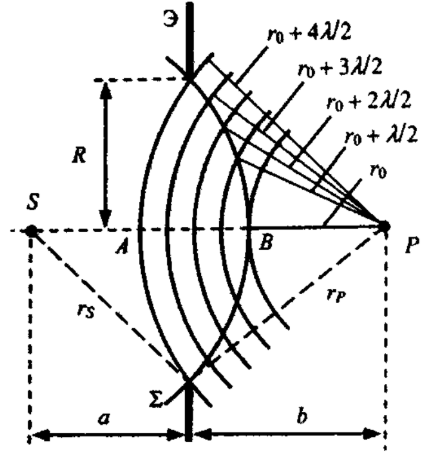
\includegraphics[width=0.4\linewidth]{img6.png}
\caption{Разбиение волнового фронта на зоны Френеля}
\label{img6}
\end{figure}

Эти сферы разбивают весь волновой фронт на кольцевые области, наз. \textit{зонами Френеля}.

\subsection{Зоны Шустера}

Рассмотрим дифракцию плоской волны на краю экрана Э, перекрывающего половину волнового фронта. Точка наблюдения $P$ расположена на экране $\text{Э}_1$, отстоящем на расстояние $h$ от экрана Э. Найдем поле в точке $P$, находящейся на расстоянии $x$ от проекции края экрана Э: при $x<0$ точка находится в области геометрической тени, в при $x>0$ - в области открытой части волнового фронта.

\begin{figure}[h]
\centering
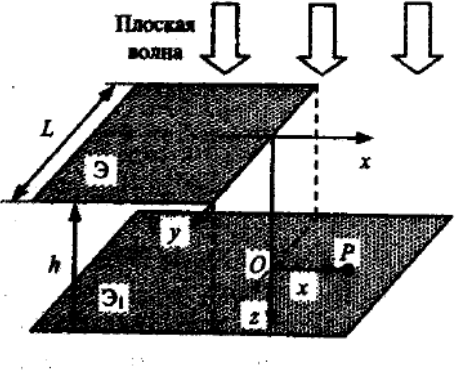
\includegraphics[width=0.4\linewidth]{img7.png}
\caption{Разбиение волнового фронта на зоны Френеля}
\label{img7}
\end{figure}

Из точки $P$ проведем серию цилиндрических поверхностей с осью, параллельной краю экрана Э и радиусами $r_n=h+n\lambda/2, \quad n=0,1,2,..$. Эти поверхности разбивают весь волновой фронт на полоски, параллельные краю, наз. зонами Шустера.

\begin{figure}[h]
\centering
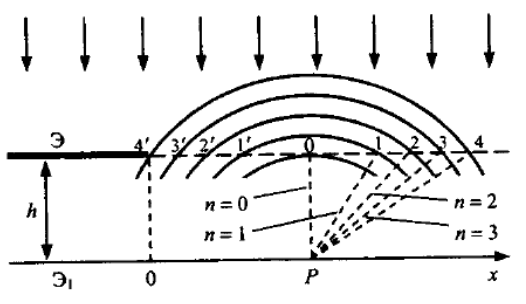
\includegraphics[width=0.4\linewidth]{img8.png}
\caption{Построение зон Шустера}
\label{img8}
\end{figure}

Ширина первой зоны: $d_1=\sqrt{(h+\lambda/2)^2-h^2}\approx\sqrt{h\lambda}$. Учитывая $n\lambda\ll h$, находим $d_n=d_1(\sqrt{n}-\sqrt{n-1})$

\subsection{Расчет дифракции с помощью интеграла Френеля}

Пусть на экран Э падает плоская волна с амплитудой $A_0$. Считая экран Э неограниченным вдоль оси $y$, обозначим координаты точки $P$ в плоскости наблюдения $\text{Э}_1$: $x_P=x, y_P=0$. Выделим на открытой части волнового фронта участок прощадью $d\sigma=dx_1dy_1$. Тогда расстояние от него до точки $P$ равно
$$
r = \sqrt{h^2+(x-x_1)^2+y_1^2}
$$
Запишем интеграл Френеля:
$$
A(P) = A(x)=\int\limits_0^\infty dx_1\int\limits_{-\infty}^\infty dy_1K(\alpha)\frac{1}{r}e^{ikr}
$$
$$
r\approx h+\frac{(x-x_1)^2+y_1^2}{2h}
$$
$$
A(x) = \frac{k}{2\pi ih}e^{ikh}\int\limits_0^\infty dx_1\int\limits_{-\infty}^\infty dy_1\exp{\Big(ik\frac{(x-x_1)^2+y_1^2}{2h} \Big)}=\frac{k}{2\pi ih}e^{ikh}\int\limits_0^\infty\exp{\Big(ik\frac{(x-x_1)^2}{2h} \Big)}dx_1\int\limits_{-\infty}^\infty\exp{\Big(ik\frac{y_1^2}{2h}dy_1 \Big)}
$$
Промежуточный результат:
$$
A(x) =a_0e^{ikh}\frac{1}{\sqrt{\pi i}}\int\limits_{-\sqrt{ax}}^\infty\exp{(i\tau^2)d\tau}
$$
Приведем результат к традиционной форме. Введем интегралы Френеля:
$$
S(u)=\sqrt{\frac{2}{\pi}}\int\limits_0^u\sin{\tau^2} d\tau, \quad C(u)=\sqrt{\frac{2}{\pi}}\int\limits_0^u \cos{\tau^2} d\tau
$$

\begin{figure}[h]
\centering
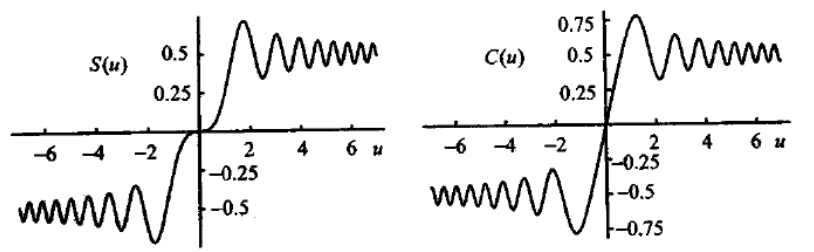
\includegraphics[width=0.4\linewidth]{img9.png}
\caption{Графики интегралов Френеля}
\label{img9}
\end{figure}

В итоге получаем:
$$
A(x)=A_0e^{ikh}\frac{1}{\sqrt{2i}}\Bigg(\Big(\frac{1}{2}+C(x\sqrt{k/2h})\Big)+i\Big(\frac{1}{2}+S(x\sqrt{k/2h})\Big)\Bigg)
$$

Для интенсивности $I=|A^2|$ получаем
$$
I = \frac{1}{2}I_0\Bigg(\Big(\frac{1}{2}+C(x\sqrt{k/2h})\Big)^2+\Big(\frac{1}{2}+S(x\sqrt{k/2h}) \Big)^2\Bigg)
$$

\begin{figure}[h]
\centering
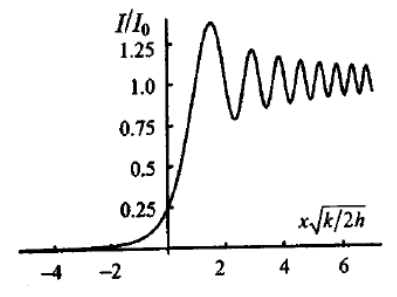
\includegraphics[width=0.4\linewidth]{img10.png}
\caption{График зависимости интенсивности излучения от координаты $x$ точки наблюдения относительно края}
\label{img10}
\end{figure}

\subsection{Спираль Корню}

Исследуем, как меняется поле в точке наблюдения в зависимости от того, какая часть волнового фронта открыта.

Пусть точка $P$ находится точно под краем: $x=0$. Если при этом ширина открытой части волнового фронта справа от $P$ конечна и равна $b$, то поле будет даваться формулой:
$$
A_1(b)=A_0e^{ikh}\frac{1}{\sqrt{\pi i}}\int\limits_0^{b\sqrt{a}}\exp{(i\xi^2)}d\xi=\frac{1}{\sqrt{2i}}A_0e^{ikh}\Big(C(b\sqrt{a})+iS(b\sqrt{a})\Big), \quad \alpha=\frac{k}{2h}
$$

Соответственно для интенсивности волны получаем:
$$
I_1(b)=\frac{1}{2}I_0\Big(C^2(b\sqrt{a})+S^2(b\sqrt{a})\Big), \quad \alpha=\frac{k}{2h}
$$

Проведенным расчетам можно дать наглядную геометрическую интерпретацию на комплексной плоскости. Введем вектор:
$$
A_1(b)=\frac{1}{\sqrt{2}}A_0\Big(C(b\sqrt{a})+iS(b\sqrt{a})\Big)
$$

Мы выбрали начало отсчета фазы волны от значения амплитуды при $b\rightarrow 0$. Этот вектор по мере изменения ширины $b$ открытой части волнового фронта поворачивается против часовой стрелки, причем его конец описывает кривую -\textit{спираль Корню}.

\begin{figure}[h]
\centering
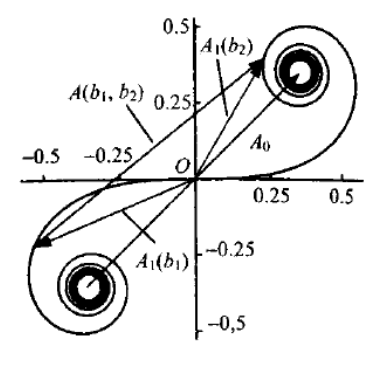
\includegraphics[width=0.4\linewidth]{img11.png}
\caption{Спираль Корню}
\label{img11}
\end{figure}

\subsection{Типы дифракции}

Пусть излучение падает на непрозрачный экран с отверстием размером $b$. Поскольку граница $n$-й зоны Френеля дается формулой $r_n=\sqrt{n\lambda h}$, то по отношению к точке наблюдения $P$ в отверстии укладывается число зон $n\sim b^2/\lambda h$. Соответственно говорят, чтопри $n\ll 1$ имеет место дифракция \textit{Фраунгофера}, при $n\sim 1$ реализуется дифракция \textit{Френеля}, а при $n\gg 1$ - \textit{геометрическая оптика}.

Величина $f=b^2/\lambda h$ наз. \textit{параметром Френеля}. Используют также \textit{волновой параметр}: $p=1/\sqrt{f}=\sqrt{\lambda h}/b$.

Условие дифракции Фраунгофера:
$$
\frac{b}{h}\ll \frac{\lambda}{b}\ll 1
$$

Расстояние, при котором отверстие имеет размер порядка одной зоны Френеля:
$$
z_\text{Д}=b^2/\lambda
$$
Эта величина наз. \textit{дифракционной длиной светового пучка}. Таким образом дифракция Фраунгофера наблюдается на расстояниях, превышающих дифракционную длину пучка.

\subsection{Дифракция Фраунгофера на щели}

Пусть плоская волна $A=A_0e^{ikz}$ падает по нормали на экран с щелью шириной $b$. Дифракцию Фраунгофера можно наблюдать в дальней зоне в виде серии полос , параллельных краю щели. Если же на пути дифрагированной волны поставить линзу, то в ее фокальной плоскости возникнет серия точек, отвечающих дифракционным максимумам.

\begin{figure}[h]
\centering
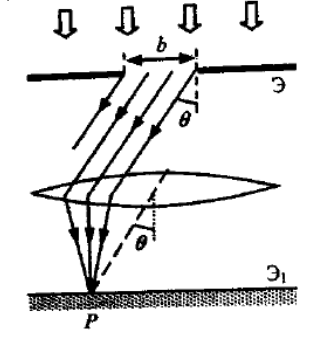
\includegraphics[width=0.2\linewidth]{img12.png}
\caption{Схема наблюдения дифракции Фраунгофера}
\label{img12}
\end{figure}

Разность хода волн от полоски с координатой $x$ и от начальной полоскии равна $\Delta =x\sin{\theta}$. Введем обозначение $u=k\sin{\theta}$.
$$
A(\theta)=\int dA\sim \frac{A_0}{b}\int\limits_{-b/2}^{b/2}e^{iux}dx=A_0\frac{\sin(ub/2)}{ub/2}
$$
Выражение для интенсивности:
$$
I(\theta)=I_m\Big(\frac{\sin{ub/2}}{ub/2}\Big)^2, \quad u=k\sin{\theta}
$$

\begin{figure}[h]
\centering
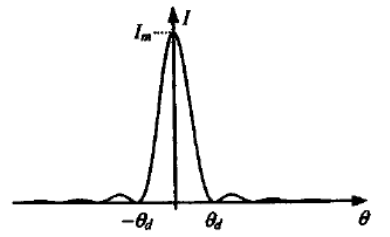
\includegraphics[width=0.4\linewidth]{img13.png}
\caption{Зависимость интенсивности излучения от направления при дифракции Фраунгофера на щели}
\label{img13}
\end{figure}

\subsection{А. Дифракция Френеля}


Схема установки для наблюдения дифракции Френеля представлена на рис. $\ref{img1}$. Свет от ртутной лампы Л, пропущенный через оранжевый светофильтр Ф со средней длиной волны $\lambda=578\text{нм}$, падает на входную щель $S_1$. Щель $S_1$ находится в фокусе \textit{коллиматора} - собирающей линзы $O_1$. Коллиматор создает параллельный пучок монохроматического света, освещающий щель $S_2$, на которой и происходит дифракция. Дифракционная картина рассматривается с помощью микроскопа M, сфокусированного на некоторую плоскость наблюдения П.

\begin{figure}[h]
\centering
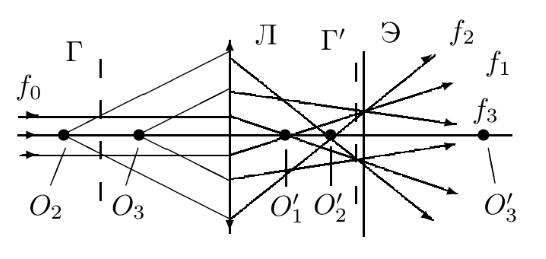
\includegraphics[width=0.8\linewidth]{img1.png}
\caption{Схема установки для наблюдения дифракции Френеля}
\label{img1}
\end{figure}

Распределение интенсивности света в плоскости наблюдения П проще всего рассчитывать с помощью \textit{зон Френеля}. При освещении щели $S_2$ параллельным пучком лучей (плоская волна) зоны Френеля представляют собой полоски, параллельные краям щели(рис.$\ref{img2}$). Результирующая амплитуда в точке наблюдения определяется суперпозицией колебаний от тех зон Френеля, которые не перекрыты створками щели. Границы зон Френеля $\xi_m$ определяется соотношением:
\begin{equation}
    \xi_m=\pm \sqrt{mz\lambda}, \quad m \in \mathbb{N}
\end{equation}
где $\xi$ отсчитывается от центра щели, $z$ - расстояние от щели до плоскости наблюдения П, а $\lambda$ - длина волны. При ширине щели $b$ ($-b/2 <\xi<b/2$) полное число открытых зон для точки наблюдения на оси равно
\begin{equation}
    m_\text{max} = \frac{b^2}{4\lambda z}
\end{equation}

\begin{figure}[h]
\centering
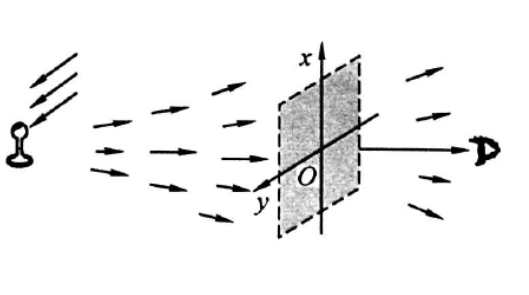
\includegraphics[width=0.2\linewidth]{img2.png}
\caption{Зоны Шустера в плоскости щели}
\label{img2}
\end{figure}

Разделение волнового фронта на зоны Френеля производится так, чтобы излучение от соседних зон находилось в \textit{противофазе}. То есть, разность хода между краями соседних зон равна $\lambda/2$. Поэтому, когда открыто \textit{четное} число зон Френеля, на оси системы наблюдается $\textit{минимум}$ лифракционной картины. Если число \textit{нечетно}, в центре картины - \textit{максимум}.

Зафиксируем размер щели $b$ и посмотрим, как меняется картина в зависимости от расстояния до плоскости наблюдения $z$. Если число открытых зон Френеля велико, $m \gg 1 (z\longrightarrow 0)$, мы приходим к пределу геометрической оптики: дифракционная картина отсутствует, а размер изображения щели совпадает с шириной щели $b$. Дифракционная картина наблюдается только в узкой полосе вблизи границ щели. При $m \sim 1$ на щели наблюдается сложная картина из небольшого числа дифракционных полос. При дальнейшем удалении ($m\ll1, z\longrightarrow\infty$) дифракционная картина начинает упрошаться и расширятсья, переходя в режим \textit{Фраунгофера} - ззатухающие по интенсивности эквидистантные полосы с характерынм угловым размером центральной полосы $\lambda/b$.

Амплитуду света в произвольной точке плоскости наблюдения можно определить графически с помощью векторной диаграммы - \textit{спирали Корню}.

Распределение амплитуд в режиме дифракции Френеля($m\sim1$) довольно сложно. Но если число открытых зон Френеля больше единицы и близко к целому $m=2,3,4,..$, то в картине можно довольно четко выделить $m-1$ темных полос, заполняющих изображение щели. 

\subsection{Б. Дифракция Фраунгофера на щели}
На значительном удалении от щели, когда выполнено условие $m\ll 1$(то есть шиирна щели становится значительно меньше первой зоны Френеля, $b\ll\sqrt{\lambda z}$), изображение щели размывается и возникает дифракционная картина, называемая дифракцией Фраунгофера.

Дифракцию Фраунгофера можно наблюдать той же установке, что и дифракцию Френеля (рис.$\ref{img1}$). Однако при обычных размерах установки дифракция Фраунгофера возникает только при очень узких щелях. Поскольку работать с тонкими щелями неудобно, для наблюдении дифракции Фраунгофера к схеме добавляется объектив $O_2$ (рис.\ref{img3}).

\begin{figure}[h]
\centering
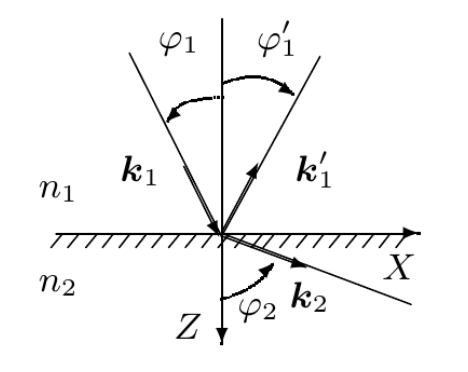
\includegraphics[width=0.8\linewidth]{img3.png}
\caption{Схема установки для наблюдения дифракции Фраунгофера на щели}
\label{img3}
\end{figure}

Дифракционная картина наблюдается в фокальной плоскости объектива $O_2$. Поскольку объектив не вносит дополнительной разности хода между интерферирующими лучами (\textit{таутохронизм} тонкой линзы), в его фокальной плоскости наблюдается неискаженная дифракционная картина Фраунгофера, соответствующая бесконечно удаленной плоскости наблюдения.

При дифракции Фраунгофера в центре поля зрения наблюдается дифракционный макксимум (светлая полоса). Сбоку от нее наблюдаются чередующиеся минимумы и максимумы с довольно быстро затухающей интенсивностью. Направление на минимумы при малых углах $\theta$ определяется соотношением 
\begin{equation}
    \theta_n^{min} = n\frac{\lambda}{b}, \quad n=\pm1, \pm2,..
\end{equation}
где $b$ - ширина щели. Каждому значению угла $\theta$ соответствует точка в плоскости объектива с фокусным расстоянием $f_2$, отстоящая от оптической оси на расстоянии 
\begin{equation}
    X_n=f_2\tan{\theta_n} \approx f_2\theta_n
\end{equation}

Измеряя зависимость $X$ от $n$ или расстояние между полосами $\Delta X$, можно определить ширину щели $S_2$.

\subsection{В. Дифракция Фраунгофера на двух щелях}
Схема для наблюдения дифракции Фраунгофера на двух щелях изображена на рис.$\ref{img4}$. По сравнению с рис.$\ref{img3}$ в ней щель $S_2$ заменена на экран Э с двумя щелями. При этом щель $S_2$ установлена вместо входной щели $S_1$.

\begin{figure}[h]
\centering
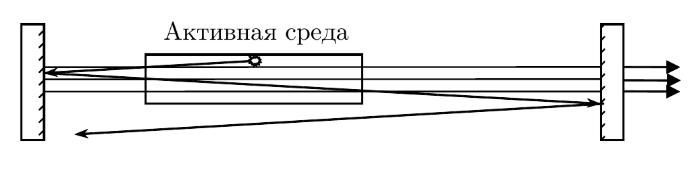
\includegraphics[width=0.8\linewidth]{img4.png}
\caption{Схема для наблюдения дифракции Фраунгофера на двух щелях}
\label{img4}
\end{figure}

Результат дифракции на двух щелях можно представить как интерференцию дифракционных картин от каждой щели. Если входная щель достаточно узка, то дифракционная картина в плоскости П подобна той, что получалась при дифракции на одной щели, однако теперь для картина испещрена рядом дополнительных узких полос. Наличие этих полос объясняется суперпозицией (интерференцией) световых волн, приходящих в плоскость наблюдения через разные щели экрана Э. В центре главного дифракционного максимума располагается светлая полоса. Светлая интерференционная полоса наблюдается также, когда разность хода кратна длине волны. Угловая координата $\theta_n$ интерференционного максимума $n$-го порядка определяется соотношением:
\begin{equation}
    \theta_nd=n\lambda, \quad n=\pm1, \pm2,..
\end{equation}
где $d$ - расстояние между щелями. Линейное расстояние $\delta x$ между соседними интерференционными полосами в плоскоти П равно поэтому
\begin{equation}
    \delta x = f_2\frac{\lambda}{d}
\end{equation}

На рис. $\ref{img4}$ показано распределение интенсивности в фокальной плоскости объектива $O_2$. Штриховой линией изображено распределение интенсивности при дифракции света на одиночной щели. Поскольку полная угловая ширина главного дифракционного максимума равна $2\lambda/D$, где $D$ - ширина отдельной щели, то на нем укладывается
\begin{equation}
    N = \frac{2d}{D}
\end{equation}
темных интерфереционных полос.

При дифракции света на двух щелях четкая система интерференционных полос наблюдается только при достаточно узкой ширине входной щели, которую можно рассматривать как протяженный источник света размером $b$. Для наблюдения интерференции необходимо, чтобы расстояние $d$ между щелями не превышало \textit{радиуса когерентности}:
\begin{equation}
    d \leq \rho_\text{ког} \approx \frac{\lambda}{b}f_1
\end{equation}

Таким образом, по размытию интерфереционной картины можно оценить размер источника $b$.

\subsection{Г. Влияние дифракции на разрешающую способность оптического инструмента}

Линзы $O_1$ и $O_2$ (без щели $S_2$) создают в плоскости П изображение щели входной $S_1$, рассматриваемое в микроскоп М. Таким образом, пара линз $O_1$, $O_2$ и микроскоп в совокупности может рассматриваться как некий \textit{оптический инструмент}. При этом входная щель $S_1$ и коллиматор $O_1$ создают модель далекого предмета, а объектив $O_2$ и микроскоп М составляют "зрительную трубу", наведенную на этот предмет.

\begin{figure}[h]
\centering
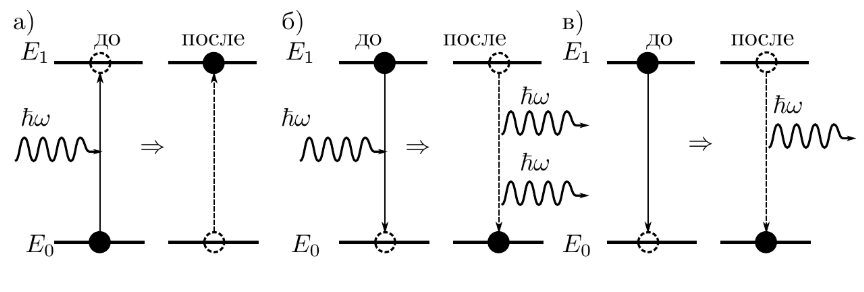
\includegraphics[width=0.8\linewidth]{img5.png}
\caption{Схема для исследования разрешающей способности оптического инструмента}
\label{img5}
\end{figure}

Если перед объективом $O_2$ зрительной трубы расположить щель $S_2$, то изображение объекта будет \textit{искажено дифракцией} на щели $S_2$. Чем меньше ширина $b$ этой щели, тем сильнее искажение. Качественной характеристикой этих искажений может служить минимальное угловое расстояние $\varphi$ между точками рассматриваемого предмета, которые воспринимаются как \textit{раздельные}.

В качестве предмета будем использовать экран Э с двумя узкими щелями. ПУсть расстояние между щелями равно $d$. Тогда от каждой из щелей экрана на щель $S_2$ будут падать два параллельных пучка света, составляющих между собой угол 
\begin{equation}
    \varphi \approx\frac{d}{f_1}
\end{equation}

Угловая ширина $\Delta \varphi$ каждого изображения определяется дифракцией света на щели $S_2$. В режиме дифракции Фраунгофера полуширина центрального дифракционного максимума равна $\Delta \varphi \sim \lambda/b$, где $b$ - ширина щели $S_2$.

Если полуширина главного дифракционного пятна превысит расстояние между центрами пятен $\Delta \varphi > \varphi$, пятна от двух щелей сольются в одно и по виду дифракционной картины будет трудно определить, представляет ли собой исчтоник двойную или одиночную щель. Это условие разрешения двух изоюражений наз. \textit{критерием Рэлея}. Щели можно считать различимыми, если
\begin{equation}
    \frac{\lambda}{b} < \frac{d}{f_1}
\end{equation}

\section{Ход работы}
\subsection{Дифракция Френеля}

\begin{enumerate}
    \item Настроим зрительную трубу на бесконечность. Предварительно настроим ее окуляр: поворотом глазной линзы добиваемся появления в поле зрения четкого изображения окулярной шкалы или креста, затем вращением регулировочного винта находим четкое изображение удаленного объекта. Следим, чтобы настройка винта в процессе работы не сбилась.
    \item Определяем нуль микрометрического винта щели $S_2$. Для этого глядя сквозь щель на окно или лампу, определим момент ее открытия. Повторим процедуру несколько раз, вращая винт все медленнее, и зафиксируем значение нуля. Максимальная ширина щели — около 0,4 мм; один оборот винта — 100 дел — соответствует 0,1 мм (цена деления — 0,001 мм).
    \item Собираем схему согласно рис.$\ref{img1}$
    \begin{enumerate}
        \item Включаем ртутную лампу, устанавливаем на ней светофильтр, затем вертикальную входную щель $S_1$. Открываем щель пошире и с помощью экрана или листа белой бумаги проверяем, что луч идет вдоль оптической скамьи.
        \item Устанавливаем линзу $O_1$ на расстоянии от щели $S_1$ близком к фокусному.
        \item Поставим щель $S_2$ сразу за линзой $O_1$ и закрепим. Убедимся, что щель вертикальна и равномерно освещена. Начальную ширину щели рекомендуется установить равной $\sim 0,2-0,3 \text{мм}$.
        \item Убедимся, что окуляр микроскопа настроен под наш глаз так, что его окулярная шкала видна четко.
        \item Сфокусируем микроскоп на щель $S_2$. Глядя в окуляр и немного перемещая микроскоп вдоль оптической оси, получим резкое изображение границ щели $S_2$.
    \end{enumerate}
    \item Проверим, что при небольшом удалении микроскопа от щели на ярком фоне геометрического изображения щели появляются узкие темные дифракционные полосы, количество которых уменьшается по мере удаления микроскопа.
    \item Попытаемся улучшить контрастность картины. Она зависит от ширины щели $S_1$, от центрировки линзы $O_1$, от равномерноести освещения щелей и их параллельности.
    \item Добившись наибольшей четкости и контрастности дифракционной картины, снова найдем резкое изображение щели. Запишем начальное положение микроскопа - координату по шкале продольной линейки, расположенной на оптической скамье.

    $z_0=692\text{мм}\pm 1\text{мм}$
    \item Постепенно отодвигая микроскоп от щели $S_2$, заметим по шкале положение микроскопа, при котором на фоне щели видна одна темная полоса (n=1). Смещение микроскопа от первоначального положения дает веичину $z$ - расстояние от щели до плоскости наблюдения. Если это расстояние слишком мало, следует увеличить ширину щели $S_2$ и снова поработать над контрастностью картины.
    \item Приближая микроскоп к щели, измерим зависимость координаты микроскопа $z$ от числа $n$ наблюдаемых темных полос.
    \begin{table}[h!]
    \centering
    \begin{tabular}{||c|c|c|c||}
    \hline
        $n$ & $z$, мм & $\Delta z$, мм & $\sigma_z$, мм  \\
        \hline
        1 & 671 & 21 & 1 \\
        2 & 681 & 13 & 1 \\
        3 & 685 & 10 & 1 \\
        4 & 687 & 7 & 1 \\
        5 & 689 & 5 & 1 \\
        6 & 690 & 3 & 1 \\
        \hline
    \end{tabular}
    \end{table}

    \item Измерим ширину $b$ щели $S_2$, используя сначала окулярную шкалу микроскопа, а затем микрометрический винт поперечных салазок микроскопа.
    
    $14\text{дел} * 0.02\text{мм} = (0.28\pm0.02)\text{мм}$ - по шкале микроскопа

    $0.305-0.037 = (0.268\pm0.001)\text{мм}$ - по микрометрическому винту

    \item Вновь сфокусируем микроскоп на щель. При небольшом удалении микроскопа от щели у ее краев появляются узкие частые полосы. Это дифракция на краю экрана.

    Наблюдаем узкие светлые полосы лишь вблизи краев щели, по всей ширине щели темные полосы, сливающиеся в единую широкую темную полосу.
    \item Закрепляем микроскоп на скамье и следим за изменением дифракционной картины при уменьшении ширины $b$ щели $S_2$.

    При открытии щели появляется больше темных полос, но они уже. Если открыть щель до конца, темные полосы станут практически прозрачными(дифракция пропадает). При уменьшении ширины щели, уменьшается количество темных полос, при этом они четче и шире.
    \item Подбираем координаты так, чтобы зависимость расстояния до щели $z$ от числа открытых зон Френеля $m$ была линейной. Построим график зависимости и по критерию хи-квадрат убедимся в том, что экспериментальные точки могут быть аппроксимированы прямой линией. По наклону наилучшей прямой определим ширину щели $b$.

    \begin{figure}[h]
    \begin{center}
        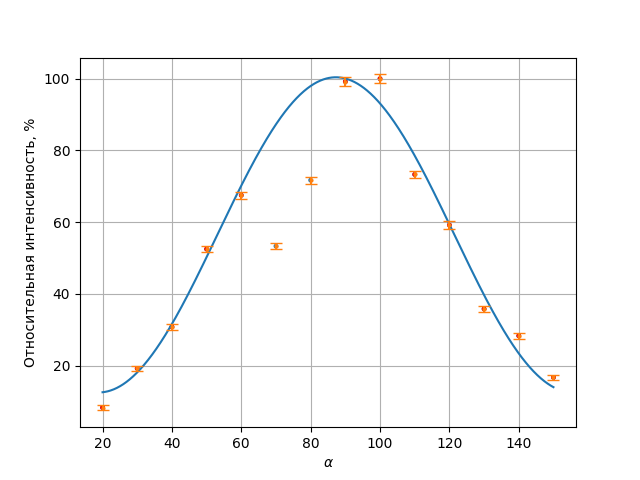
\includegraphics[width=0.8\linewidth]{graph1.png}
    \end{center}
    \caption{Зависимость $z(\frac{1}{m})$}
    \label{graph1}
    \end{figure}

    $$
    m = \frac{b^2}{4\lambda z} \rightarrow{k=\frac{b^2}{4\lambda}}\rightarrow b = 2\sqrt{k\lambda}
    $$
    где $\lambda=58\cdot10^{-5}\text{мм}$ - длина волны желтого света.
    $$
    b = 2\sqrt{22.42\cdot58\cdot10^{-5}} = 0.23\text{мм}
    $$
    $$
    \sigma_b = b\sqrt{\Big(\frac{1}{2}\frac{\sigma_k}{k}\Big)^2}=0.23\cdot\sqrt{\Big(\frac{1}{2}\frac{1.02}{22.42}\Big)^2} = 0.01\text{мм}
    $$

    \begin{center}
        \boxed{b=(0.23\pm0.01)\text{мм}, (\varepsilon=4.35\%)}
    \end{center}
    
\end{enumerate}

\subsection{Дифракция Фраунгофера}
\begin{enumerate}
    \item Не разбирая схемы, добавляем к ней линзу $O_2$. Ставим линзу $O_2$ между щелью $S_2$ и микроскопом.
    \item Настраиваем микроскоп на фокальную плоскость П линзы. Для этого временно снимаем со скамьи щель $S_2$ и убедимся, что свет проходит через центры линз и попадает на объектив микроскопа. Перемещая микроскоп вдоль скамьи, находим резкое изображение щели $S_1$. 
    \item Возвращаем щель $S_2$ между линзами и подбираем ее ширину так, чтобы в поле зрения микроскопа появилась дифракционная картина.
    \item Измеряем с помощью окулярной шкалы микроскопа координаты $x_m$ нескольких дифракционных максимумов.
    
    \begin{table}[h!]
    \centering
    \begin{tabular}{||c|c|c|c||}
    \hline
        $n$ & $x_m$, дел & $x_m$, мм & $\sigma_x$, мм \\
        \hline
        0 & 0 & 0 & 0.02 \\
        1 & 11 & 0.22 & 0.02 \\
        -1 & -11 & -0.22 & 0.02 \\
        2 & 22 & 0.44 & 0.02 \\
        -2 & -21 & -0.42 & 0.02 \\
        3 & 28 & 0.56 & 0.02 \\
        -3 & -27 & -0.54 & 0.02 \\
        \hline
    \end{tabular}
    \end{table}

    Ширина щели $b$ щели $S_2$ по микрометрическому винту: $0.305-0.015 = 0.29\text{мм}\pm0.02\text{мм}$

    Фокусное расстояние $f_2$ линзы $O_2$: $10\text{см}$
    \item Убедимся, что смещение щели $S_2$ в боковом направлении не приводит к сдвигу дифракционной картины.


    \item Наблюдаем, как изменяется масштаб дифракционной картины при уменьшении ширины $b$ щели $S_2$.

    При уменьшении щели увеличивается число дифракционных макисмумов и картина становится четче.
    \item Построим график зависимости положений $x_m$ экстремумов дифракционной картины от их номера $m$. Апроксимируем зависимость прямой, по ее наклону находим ширину щели $b$.

    \begin{figure}[h]
    \centering
    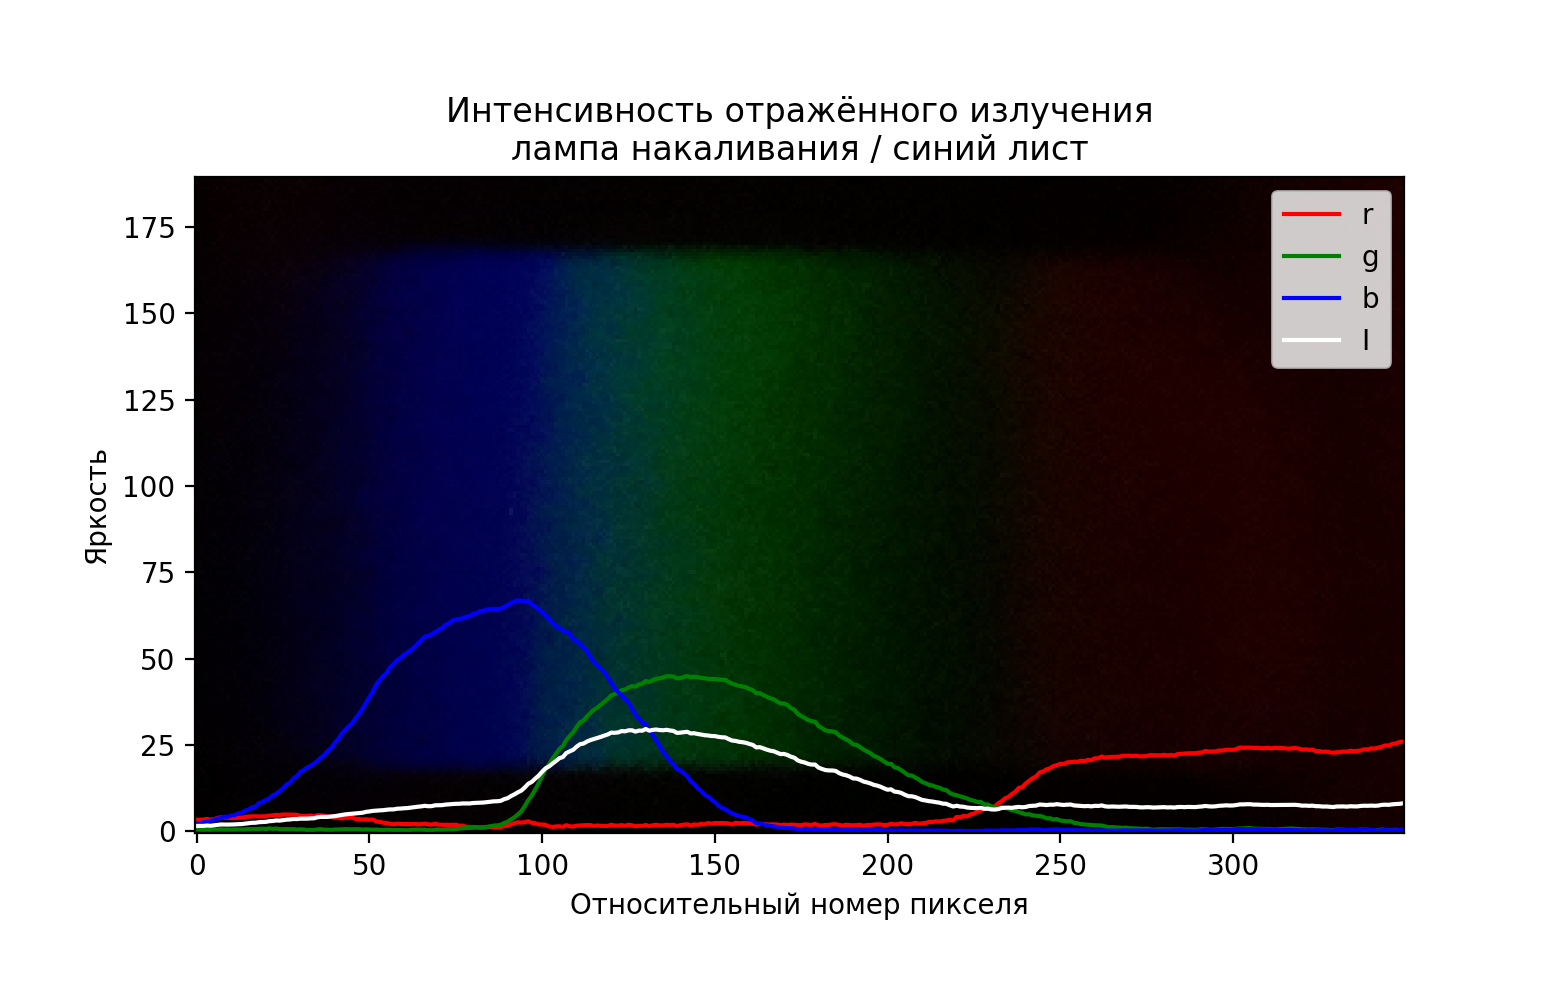
\includegraphics[width=0.8\linewidth]{graph2.png}
    \caption{Зависимость координаты дифракционного минимума от его номера}
    \label{g2}
    \end{figure}

    $x_m = f_2\frac{\lambda}{b}m\Longrightarrow b = f_2\cdot\lambda/k = 100 \cdot 58\cdot10^{-5} / 0.195=0.297\text{мм}$

    где $\lambda = 58\cdot10^{-5}\text{мм}$ - длина волны желтого света.

    $\sigma_b = b\sqrt{\Big(\frac{1}{2}\frac{\sigma_k}{k}\Big)^2} \Longrightarrow \sigma_b = 0.297\cdot\sqrt{\Big(\frac{1}{2}\frac{0.011}{0.195}\Big)^2}=0.012\text{мм}$
    \begin{center}
    \boxed{b=(0.297\pm0.012)\text{мм}, (\varepsilon=4.04\%)}    
    \end{center}
    
    Сравниваем результат с прямым измерением по микрометрическому винту. Отклонение составляет $\Delta=\frac{297-290}{290}\cdot100\%\approx2.4\%$
\end{enumerate}

\subsection{Дифракция Фраунгофера на двух щелях}
\begin{enumerate}
    \item Не перемещая линз и микроскопа в установке, убираем входную щель $S_1$ и устанавливаем на ее место щель с микрометрическим винтом $S_2$. Слегка передвигая щель $S_2$ вдоль скамьи, найдем в микроскопе резкое изображение новой входной щели.
    \item Поставим между линзами экран Э с двойной щелью. В области главного дифракционного максимума должна появиться система равноотстоящих темных и светлых полос. Центрировкой системы и подбором ширины входной щели добиваемся наибольшей четкости дифракционной картины.
    \item Измеряем расстояние $\delta x$ между минимумами интерференционной картины. Для этого можно с помощью микрометрического винта поперечных салазок микроскопа определяем координаты самых удаленных друг от друга темных полос внутри центрального максимума и подсчитаем число светлых промежутков между ними.

    $\delta x = \frac{0.22\text{мм}}{7}=(0.031\pm0.001)\text{мм}$
    \item Посчитаем полное число светлых интерференционных полос в пределах главного (центрального) максимума:

    $N =7$
    \item Исследуем влияние размера источника на видность интереференционной картины. Для этого, расширяя входную щель $S$, подбираем такую ширину щели $b_0$, при которой наступает первое исчезновение интерференционных полос.

    $b_0 = 0.305-0.07=(0.235\pm0.001)\text{мм}$
    \item Убедимся, что при дальнейшем увеличении входной щели картина вновь появляется но она менеее контрастна. Определим соотвествующую ширину входной щели $b_1$:

    $b_1 = 0.305-0.216 = (0.089\pm0.001)\text{мм}$
    \item Фокусное расстояние: $f_1 = 10\text{см}$ и $f_2=7\text{см}$
    \item Ширину двойных щелей $D$ и расстояния между ними $d$ можно измерить с помощью микроскопа.
    \item По расстоянию $\delta x$ между полосами рассчитаем расстояние между щелями $d$.

    $\delta x=f_2\frac{\lambda}{d} \Leftrightarrow d=f_2\frac{\lambda}{\delta x} \Longrightarrow d=70\cdot\frac{58\cdot10^{-5}}{0.031}=1.29\text{мм}$

    \item Сравним наблюдаемое число полос в главном максимуме с теоретическим

    $N_\text{теор} = \frac{2d}{D} = 6\quad N_\text{практ} = 7$

    \item Сравним измеренную ширину $b_0$ входной щели $S$ с расчетом по формуле: 

    $d \leq\rho_{\text{ког}} \approx \frac{\lambda}{b_0}f_1 \Longleftrightarrow 1.29\leq\frac{58\cdot10^{-5}}{0.235\cdot10^{-3}}\cdot100=246$ - выполняется!

    Рассчитаем ширину $b_1$, при котором изображение должно опять появиться. Для этого рассмотрим предельный случай:

    $d =\frac{\lambda}{b_1}f_1 \Longleftrightarrow b_1=\frac{\lambda}{d}f_1 \Longrightarrow b_1=\frac{58\cdot10^{-5}}{1.29}\cdot100=0.045\text{мм}$

    Полученное значение совпадает по порядку величины с измеренным.
\end{enumerate}

\subsection{Влияние дифракции на разрешающую способность оптического инструмента}
\begin{enumerate}
    \item Собираем схему согласно рис.5. Для этого, не меняя положения линз и микроскопа, убираем входную щель $S$ и ставим на ее место экран Э с двойной щелью. Перемещая экран вдоль оси системы получаем в поле зрения микроскопа четкое, симметричное изображение двойного источника.
    \item Устанавливаем максимальную ширину щели $S_2$ и ставим ее между линзами $O_1$ и $O_2$. Постепенно уменьшая ее ширину $b$, наблюдаем за ухудшением качества изображения двойной щели в микроскоп.
    \item Подбираем ширину $b_0$ щели $S_2$ так, чтобы изображения обеих щелей почти сливались, но все-таки еще воспринимались раздельно.

    $b_0 = 0.305-0.155=(0.150\pm0.001)\text{мм}$
    \item Поставим двойную щель непосредственно перед микроскопом и измеряем с помощью микрометрического винта поперечных салазок микроскопа расстояние $d$ между щелями и ширину каждой щели $D$:

    $d = 35 \cdot 0.02\text{мм} = (0.70\pm0.02)\text{мм}$
    
    $D = 11 \cdot 0.02\text{мм} = (0.22\pm0.02)\text{мм}$
\end{enumerate}

\section{Выводы} 

В данной лабораторной работе мы исследовали явление дифракции Фринеля и Фраунгофера на одной и двух щелях, проверили теоретические соотношения для положения максимумов при дифрауции Френеля и Фраунгофера.

В ходе работы мы научились юстировать сложные оптические системы, работать с линзами и дифракционными щелями, фильтром света.

Исследовали зависимость расстояния до щели $z$ от числа открытых зон Френеля $m$, с помощью графика определили размер щели $b$; исследовали зависимость положения экстремумов $x_m$ от их номера $m$, с помощью графика определили размер щели $b$.

Полученные значения совпадают по порядку величины с теоретическими

\end{document}
